\chapter{Background}
\label{cha:background}
The Stratosphere is a layer of the Earth's atmosphere characterised by increasing temperatures with height. This feature distinguishes it from the lowest layer of the atmosphere, the troposphere, and makes it stable to vertical convection. As a result, the stratosphere exhibits significantly different dynamical behaviour to the troposphere. The stratosphere is bounded by the tropopause from below and the stratopause above. The height of these bounds vary latitudinally with tropopause heights ranging from  $\sim$17-18$km$ at the equator to $\sim$6$km$ near the polar regions. While the stratosphere and troposphere are characterised separately, current understanding of atmospheric dynamics incorporates elements of coupling between the layers. This chapter outlines the key points of this understanding including dynamics of the polar and equatorial stratosphere, stratosphere-troposphere coupling as well as surface variability relevant to the stratosphere. It also introduces the time variability of dynamical features in the stratosphere, a key theme in the work presented in this thesis. 

\section{The Stratospheric Polar Vortex}
\label{sec:polar_vortex}
During Northern Hemisphere (NH) winter, the NH polar stratosphere is plunged into polar night. As a result, it experiences a net cooling effect through emission of longwave infrared radiation to space and the absence of shortwave solar radiation available for absorption. This significant cooling increases the meridional temperature gradient ($\frac{\partial T}{\partial y}$) between the polar region and the tropics. This causes an increase in the vertical shear of zonal wind according to the thermal wind balance relation,

\begin{equation} \label{eq:thermal_wind}
\frac{\partial u_g}{\partial z} = -\frac{R}{f H}\frac{\partial T}{\partial y},
\end{equation}

where $u_g$ is the geostrophic zonal wind velocity (the wind resulting in a balance between Coriolis and pressure gradient forces), $z$ is the height coordinate, $R$ is the specific gas constant ($R = 8.31JK^{\text{-} 1}mol^{\text{-} 1}$) and $H$ is the atmospheric scale height, the gain in altitude which leads to a reduction in atmospheric pressure by a factor of $e$ given by $H = RT_r/g$ (g = acceleration due to gravity and $T_r$ is a reference temperature). $f$ in equation \ref{eq:thermal_wind} is the Coriolis parameter under a beta plane approximation which is given by

\begin{equation} \label{eq:beta_plane_approx}
f = f_0 + \beta y = 2 \Omega sin(\phi_0) + 2 \Omega cos(\phi_0)\frac{ y}{a},
\end{equation}

\noindent where $\phi_0$ is a reference latitude, $\Omega$ is the rotation rate of the earth and $a$ is the Earth's radius. This increase in vertical shear in $u_g$ leads to a strong, stratospheric, westerly flow circumnavigating the North Pole during boreal winter months. This feature is known as the NH polar vortex or polar night jet. Henceforth we refer to this feature as simply "the vortex".

The vortex contains a core of cold polar air in which temperatures can drop to around 200K in the lower stratosphere according to the European Centre for Medium Range Weather Forecasting (ECMWF) interim reanalysis data set (referred to as ERA-interim, \cite{Uppala2005}). Wintertime zonal wind speeds are found to reach up to approximately $70ms^{-1}$ on the 10hPa level at a latitude of 60N. Figure \ref{fig:ERAclimDJF}a shows the climatological zonal mean (averaged over all longitudes) zonal wind (ZMZW) from ERA-interim for the December-February period. It exhibits the traits set out above with a persistent zonal westerly wind above the 30hPa level and northward of $\sim$20$^\circ$N. The troposphere exhibits two subtropical westerly jets which show lower peak magnitude winds of around 30$ms^{-1}$ on approximately 90hPa level. Also included is figure \ref{fig:ERAclimDJF}b showing the seasonal cycle in daily winds at 60N on the 10hPa level (near the edge of the vortex). On average, the vortex forms in early September and breaks down to be replaced with summer easterlies in mid-April. These winds show a large degree of variability across different seasons (figure \ref{fig:ERAclimDJF}b faint blue lines) with some seasons exhibiting anomalously strong westerly flow and others even exhibiting easterlies for a portion of the season. These effects are due to the action of atmospheric waves on the vortex and are described fully in the following section. 

\begin{figure}[h!]
\centering
    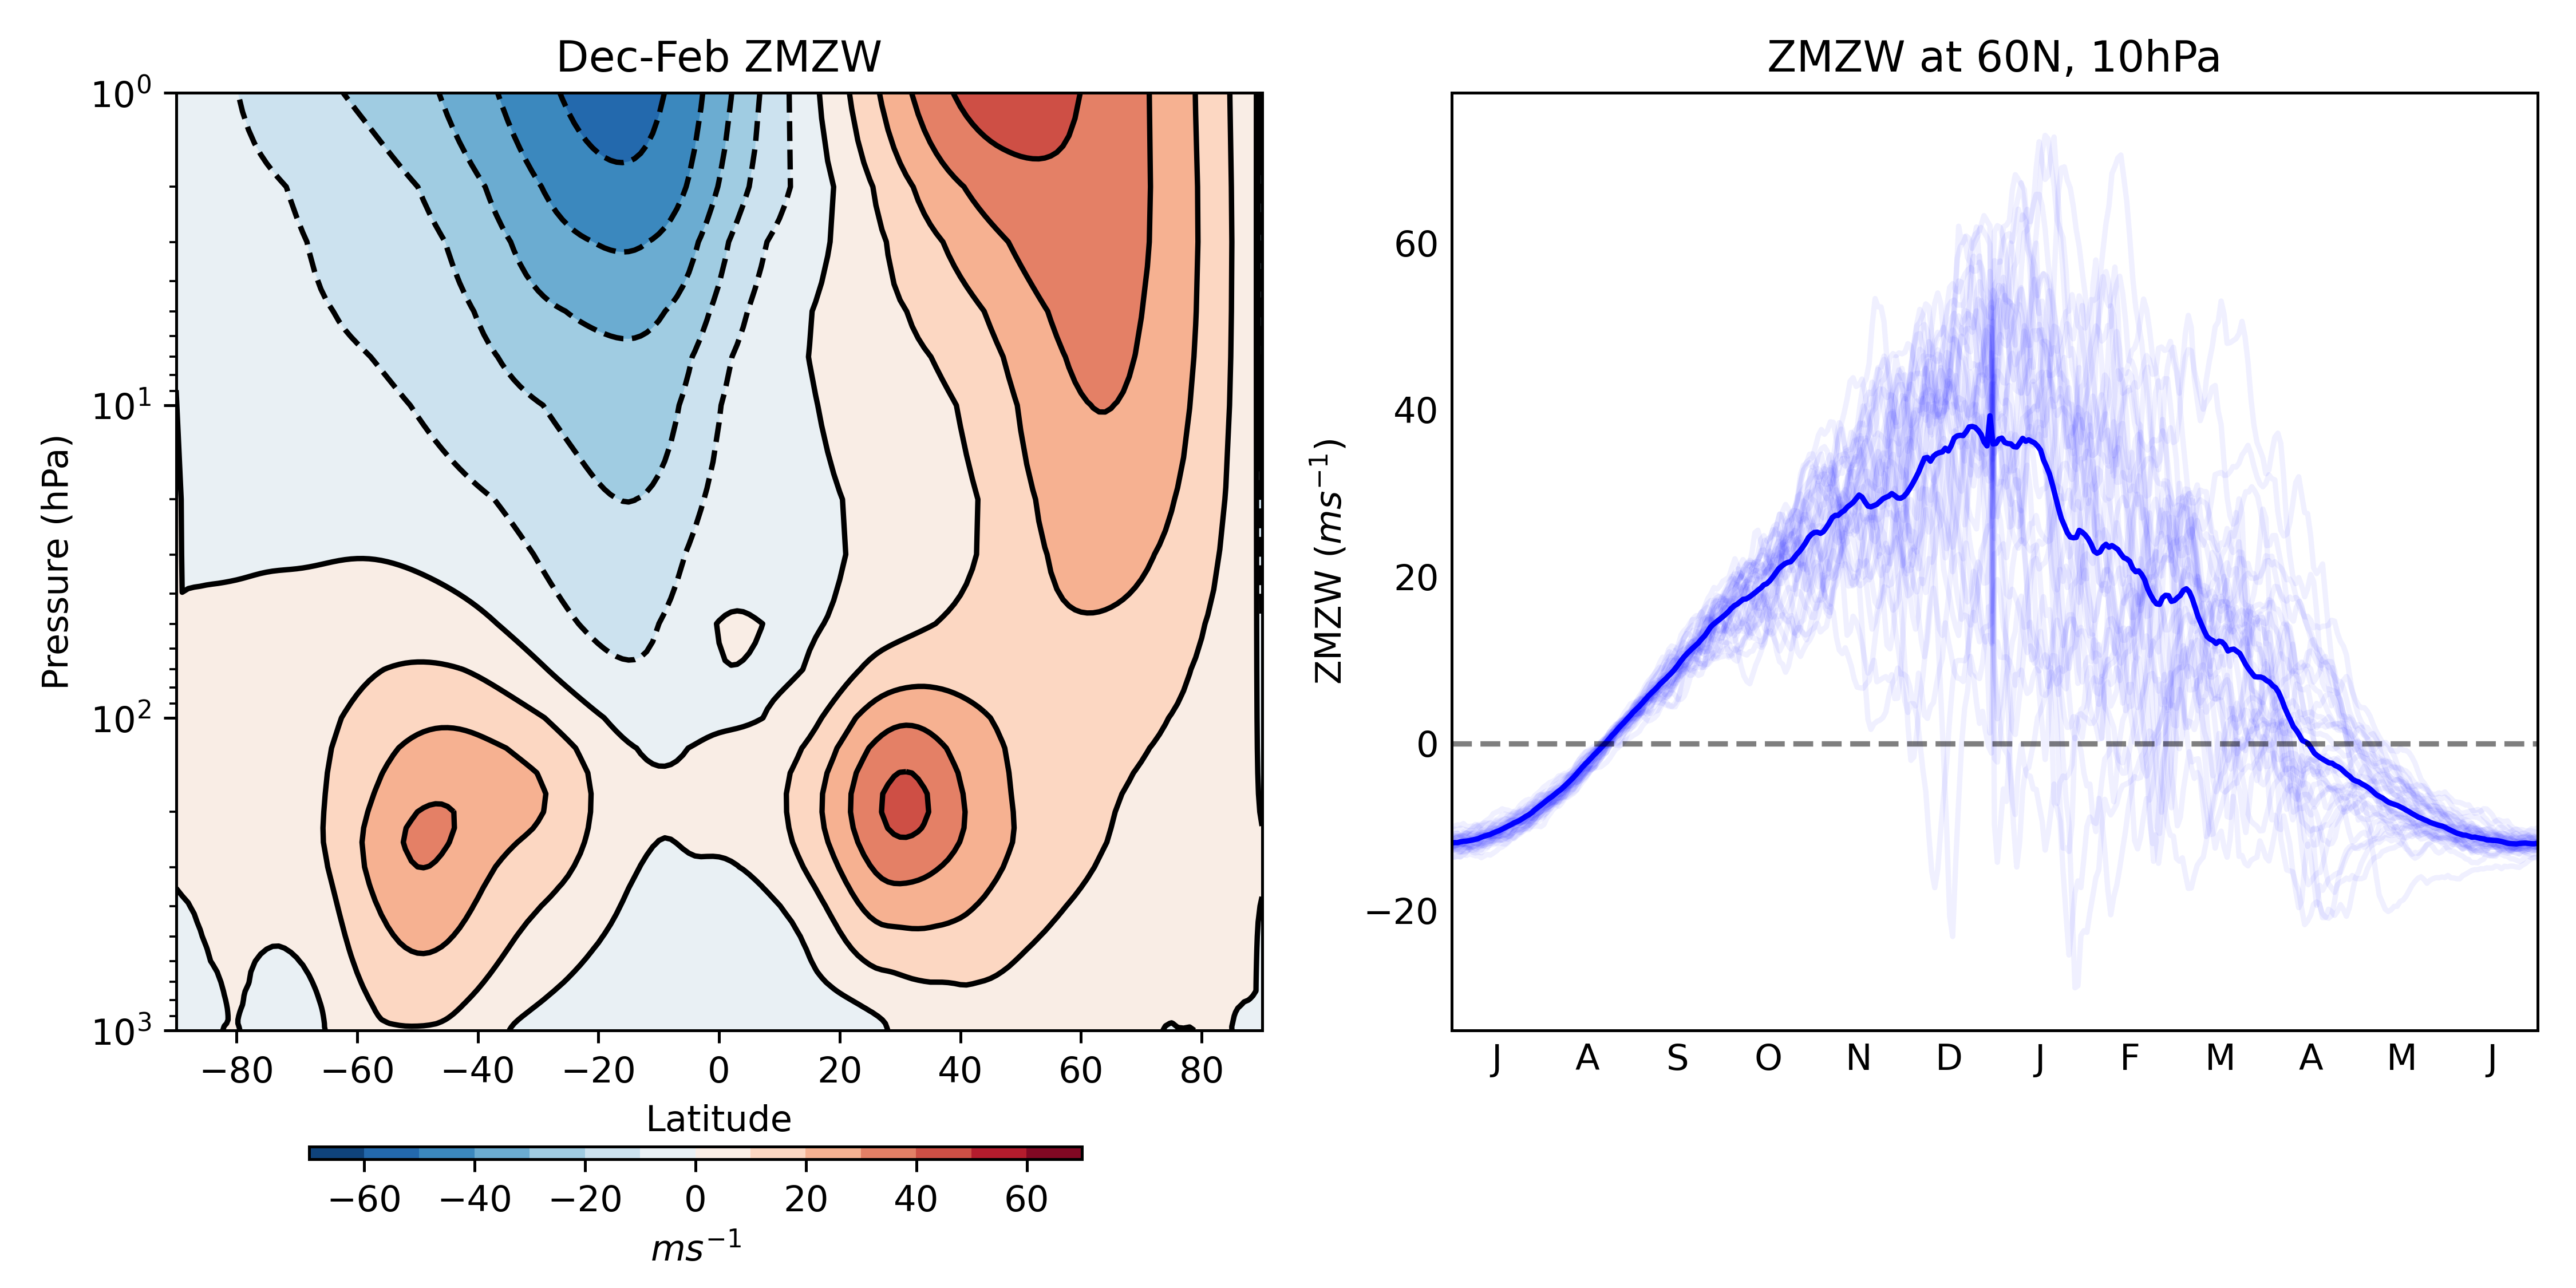
\includegraphics[width= \linewidth]{Figures/Figures-background/ZMZW_clim_cycle_ERA.png}
    \caption{\textbf{a}: Dec-Feb climatological zonal mean zonal wind from ERA-interim dataset between 1979 and 2018. \textbf{b}: Seasonal cycle in ZMZW, the zonal wind averaged over all longitudes, at 60N on the 10hPa level from the same dataset. The thick blue line indicates the seasonal cycle and faint blue lines signify winds from individual years.}
    \label{fig:ERAclimDJF}
\centering
\end{figure}

\section{Atmospheric Waves}
\label{sec:atmos_waves}
Atmospheric wave is the term generally used for deviations from the zonal mean dynamical state and these phenomena, often referred to as Rossby waves, play a key role in the variability of the vortex. These waves are forced in the troposphere by air flowing over variations in topography (orographic waves) or through other mechanisms such as interaction with convection fronts and latent heat release (non-orographic). Perturbations originating near the surface can propagate vertically into the stratosphere altering large scale circulation features via wave drag as they transfer momentum to the background flow. 

Large scale Rossby waves are known as planetary waves and exhibit wavelengths of the order of $\sim 1000km$. The propagation of these waves can be described using the Quasi Geostrophic approximation for fluid in hydrostatic balance with low ($<0.1$) Rossby number, $R_0 = U/f_0 L$, where U and L are characteristic zonal velocity and length scales respectively. Under this framework the Quasi Geostrophic Potential Vorticity (QGPV) equation states that in the absence of friction and diabatic heating, the quasi geostrophic potential vorticity, $q$, is conserved following the geostrophic wind:

\begin{equation} \label{eq-PV_conserved}
D_g q = 0
\end{equation}

\noindent where $D_g$ is the operator 

\begin{equation}\label{eq:D_g}
D_g = \frac{\partial}{\partial t} + u_g \frac{\partial}{\partial x} + v_g\frac{\partial}{\partial y} 
\end{equation}

\noindent and $q$ can be written in terms of the stream function, $\psi$, in the QGPV framework as

\begin{equation} \label{eq:QGPV}
q = f_0 + \beta y + \nabla^2 \psi + \frac{\partial}{\partial z}\bigg(\frac{f_0^2}{N_B^2} \frac{\partial \psi}{\partial z}\bigg)
\end{equation}

\noindent where $N_B$ is the Brunt–Väisälä frequency, the frequency of vertical motion of a parcel of air in a stable atmosphere. $\psi$ is related to $u_g$ and $v_g$, the zonal and meridional components of geostrophic wind by $u_g = -\frac{\partial \psi}{\partial y}$ and $v_g = -\frac{\partial \psi}{\partial x}$. Under a further approximation of small disturbances from a uniform zonal flow, $\overline{u}$, $\psi$ is given by

\begin{equation} \label{eq:Zonal_flow_SF}
\psi = -\overline{u} y + \psi '
\end{equation}

\noindent where $\psi'$ is the contribution to the stream function from the small deviation from $\overline{u}$. This approximation allows equation \ref{eq:QGPV} to be linearised to

\begin{equation} \label{eq:Linearised_QGPV}
\bigg(\frac{\partial}{\partial t} + \overline{u} \frac{\partial}{\partial x}\bigg)\Gamma \psi' + \beta \frac{\partial \psi'}{\partial x} = 0,
\end{equation}

\noindent where $\Gamma$ is the operator

\begin{equation} \label{eq:ellipse_operator}
\Gamma = \nabla^2 \psi + \frac{\partial}{\partial z}\bigg(\frac{f_0^2}{N_B^2}\frac{\partial}{\partial z}\bigg).
\end{equation}

It can be shown that this equation has wave like solutions whose vertical propagation is only supported if the following condition is satisfied:

\begin{equation} \label{eq:propagation_critera}
\overline{u} - c = \frac{\beta k}{k^2 + l^2 + \frac{f_0^2 m^2}{N_B^2}} < \overline{u}_c = \frac{\beta k}{k^2 + l^2}
\end{equation}

\noindent where $\overline{u}_c$ is a critical velocity corresponding to the background flow when $m = 0$, $c$ is the phase speed and $k, l$ and $m$ are the meridional, zonal and vertical wavenumbers of the wave respectively. Also imposing that, as $m^2 > 0$, $\overline{u} - c > 0$ as well as assuming stationary waves ($c = 0$) gives the Charney-Drazin criterion for the vertical propagation of planetary waves,

\begin{equation} \label{eq:Charney-Drazin}
0 < \overline{u} < \overline{u}_c.
\end{equation}

This result implies that vertical propagation can only occur through background westerly zonal flow with a magnitude less than some critical value, $\overline{u}_c$, which depends on the horizontal wavenumbers of the wave. More specifically, equation \ref{eq:propagation_critera} shows that smaller wave-numbers (larger wavelengths) favours greater propagation. As a result, the spectrum of waves propagating vertically from the troposphere to the stratosphere is dominated by disturbances of wavenumbers 1-3 (referred to as wave-n disturbances).  

The Charney-Drazin criterion also leads to the definition of a critical layer of the atmosphere as the layer at which the background zonal flow no longer supports propagation of a given wave (i.e. where $\overline{u} \sim \overline{u}_c$). When a wave encounters a critical layer, much of the linear dynamical behaviour proposed in equation \ref{eq:Linearised_QGPV} breaks down as the waves' amplitude grows too large to support continued propagation and it dissipates, transferring momentum to the background flow through so called wave-mean flow interactions. There therefore exists a two way interaction between the background flow and wave disturbances in the atmosphere: the magnitude of $\overline{u}$ relative to $\overline{u}_c$ dictates the propagation of waves through the troposphere into the stratosphere and waves significantly influence the background wind upon dissipation at a critical layer.

Wave-mean flow momentum deposition, which is key for understanding stratospheric dynamical variability, can be quantified via the introduction of a variable known as the Eliassen-Palm flux. In the QG framework as above, equations for the zonal mean and eddy components (deviations from the zonal mean) of the wind vector ($u, v$) and buoyancy ($b$), the vertical acceleration of air parcels due to density variations, can be expressed as 

\begin{equation} \label{eq:QG_Ubar}
\frac{\partial \overline{u}}{\partial t} = f\overline{v} - \frac{\partial}{\partial y} \overline{u'v'} + \overline{X}, 
\end{equation}

\begin{equation} \label{eq:QG_theta}
\frac{\partial \overline{b}}{\partial t} = -N^2\overline{w} - \frac{\partial}{\partial y} \overline{v'b'} + \overline{Q}, 
\end{equation}

\noindent where the overbar denotes a zonal mean quantities and deviations from this (eddy quantities) are denoted by primes. $\overline{X}$ and $\overline{Y}$ represent the dissipative forces on the flow (in this case friction and diabatic heating). Buoyancy is used in these equations as a close analogy of temperature. $b = g\frac{T - T_r}{T_r}$ where $T_r$ is a reference temperature normally defined by height. $b$ is related to the concept of reduced gravity which is important when considering vertical fluid motion. 

In order to decouple these equations, we introduce the mean residual circulation, the difference between zonal mean flow and contributions from eddy-mean flow interactions. These are known as the Transformed Eulerian Mean (TEM) meridional and vertical velocities \citep{andrewsPlanetary1976} (denoted by $^*$) and can be expressed as 

\begin{equation} \label{eq:V*}
\overline{v^*} = \overline{v} - \frac{1}{\rho_0}\frac{\partial}{\partial z} \bigg(\rho_0 \frac{\overline{v'\theta'}}{\frac{\partial{\overline{\theta}}}{\partial{z}}}\bigg)
\end{equation}\break
\begin{equation} \label{eq:W*}
\overline{w^*} = \overline{w} + \frac{\partial}{\partial y} \bigg( \frac{\overline{v'b'}}{\frac{\partial{\overline{\theta}}}{\partial{z}}}\bigg).
\end{equation}

Under these transformations the decoupled equations can be written as

\begin{equation} \label{eq:decoupled_U}
\frac{\partial \overline{u}}{\partial t} - f_0 \overline{v*} = \frac{1}{\rho_0} (\nabla \cdot F) + \overline{X}
\end{equation}

and

\begin{equation} \label{eq:decoupled_b}
\frac{\partial \overline{b}}{\partial t} + N^2 \overline{w*} = \overline{Q},
\end{equation}

where

\begin{equation} \label{eq:EP_flux}
F = -\rho_0 \overline{u'v'}\textbf{j} + f\rho_0\frac{\overline{v'\theta'}}{\frac{\partial{\overline{\theta}}}{\partial{z}}} \textbf{k}
\end{equation}

\noindent is the Eliassen-Palm flux which can be thought of as the flux of wave activity in the meridional and vertical directions (\textbf{j} and \textbf{k} represent unit vectors in the $y$ and $z$ directions) \citep{andrewsPlanetary1976}. These equations indicate that EP flux convergence ($\nabla \cdot F < 0$) signifies momentum transfer from eddies to the background flow via wave dissipation (e.g. when breaking occurs). Conversely, flux convergence ($\nabla \cdot F > 0$) indicates wave growth at the expense of momentum of the mean flow. 

\subsection{Other Atmospheric Waves} \label{sec:other_waves}
In addition to planetary scale Rossby waves outlined in previous sections, other types of wave play a vital role in stratospheric variability. Gravity waves arise due to buoyancy variations and, similarly to planetary waves, can be forced through airflow over variations in topography (orographic) or convection fronts (non-orographic). These waves exhibit length scales significantly shorter than planetary waves ($\sim xxxm$) and are often not explicitly represented in general circulation models (GCMs) due to horizontal resolution issues. Instead their effects are parameterised and appear in the dissipative force term ($\overline{X}$) in equation \ref{eq:QG_Ubar}.

Kelvin waves occur when air is trapped between regions in which Coriolis force terms act in opposite directions. In these regions, geostrophic balance does not apply and the waves exhibit a westerly phase velocity. Dissipation of these waves contributes westerly momentum to the background flow. Finally, Rossby-gravity waves exhibit different behaviour for small and large length scales (or horizontal wave number, $k$). For small $k$ (large length scale), they reduce to Rossby wavelike disturbances, similar to planetary scale Rossby waves outlined in the previous section in which variations in Coriolis parameter with latitude act as the restoring force. For large $k$ (shorter length scales), they behave as gravity waves (those for which the restoring force is gravity). Rossby-gravity waves typically have easterly phase velocity and contribute easterly momentum to background flow upon dissipation \citep{andrewsPlanetary1976}.

\section{Sudden Stratospheric Warmings}
\label{sec:SSWs}
While the vortex generally exhibits strong, westerly flow over boreal winter, it can be significantly disrupted and even reversed on sub-seasonal timescales
(see individual season winds on figure \ref{fig:ERAclimDJF}b). This reversal occurs due to the dissipation of planetary waves which transfer easterly momentum on the background flow. If this wave forcing is large enough such that the vortex becomes significantly disrupted (and reversed) an event known as a sudden stratospheric warming (SSW) occurs. Such events are named as they are associated with significant and rapid increases in middle atmosphere NH polar cap temperature ($\sim50K$ over a few days) which is achieved by the descent of air at polar latitudes, causing an adiabatic increase in temperature. These events were first observed in radiosonde data in \cite{scherhagExplosionsartigen1952}. In observation based datasets SSWs occur at an average rate of approximately 6.2 events per decade \citep{butlerSudden2017} and represent one of the largest modes of interannual variability in the NH stratosphere.

\cite{matsunoDynamical1971b} was the first work to introduce a dynamical model linking the action of planetary waves and the occurrence of SSWs. The framework developed by this work is still largely accepted today and describes the mechanisms involved in the life cycle of an SSW as follows: First, a burst of planetary wave activity is generated in the troposphere through a combination of airflow of topography and convection fronts. Waves subsequently propagate into the stratosphere in accordance with the Charney-Drazin criterion (equation \ref{eq:Charney-Drazin}). When these waves encounter a critical layer (normally one which exhibits stronger westerlies than $\overline{u}_c$ as the undisturbed vortex is strong) these waves break and dissipate easterly momentum to the background zonal flow. As a result, the westerly vortex decelerates and, if stratospheric conditions are appropriate or the planetary wave activity is strong enough, even reverses. As a result, new critical layers are formed (where $\overline{u} = 0$) at a level below that of the original reversal. Subsequent waves now dissipate and can act to reverse the background flow at this lower critical layer. This process repeats and the critical layers can descend into the lower stratosphere. Once the critical layer lies near the tropopause, planetary waves are effectively prevented from entering the stratosphere stopping further deceleration of the vortex. With wave driving of the vortex prevented, radiative cooling of the stratosphere subsequently brings polar cap temperatures back down and the strong westerly flow of the vortex recovers.

While this framework of dynamical processes involved in SSWs is relatively well accepted, there are contrasting hypotheses regarding the triggering mechanisms which initiate events. The primary mechanism suggested as the trigger is a rapid injection of wave activity from the troposphere which is large enough to significantly disrupt the vortex \citep{matsunoDynamical1971b, limpasuvanLife2004b, manneyAura2009b, nishiiModulations2009b, kuttippurathComparative2012b}. An alternative hypothesis is that the state of the stratosphere itself also plays a key role in triggering events. Many studies support this phenomenon and have shown SSWs preceded by moderate levels of wave driving from the troposphere which is subsequently amplified through non-linear resonance mechanisms with the stratospheric background flow \citep{eslerExcitation2005b, scottInternal2006b, eslerStratospheric2011a}.

The framework of \cite{matsunoDynamical1971b} provides a mechanism by which SSWs occur through the interaction between planetary waves and the zonal mean background flow. However, further studies show that as well as zonal mean disturbance, the 2D geometry of the vortex (i.e. the latitude-longitude plane on a given pressure level) is altered significantly during these events and this provides a method of event classification \citep{lehtonenObserved2016b, Mitchell2011a, Seviour2013}. During events, the vortex can either be displaced from its stable configuration, an example of which is provided in figure \ref{fig:GPH_schematic}a, to one in which its centroid shifts to a lower latitude (figure \ref{fig:GPH_schematic}b) or split into two daughter vortices each of which exhibits a core of high PV air (figure \ref{fig:GPH_schematic}c). 
\begin{figure}[h!]
\centering
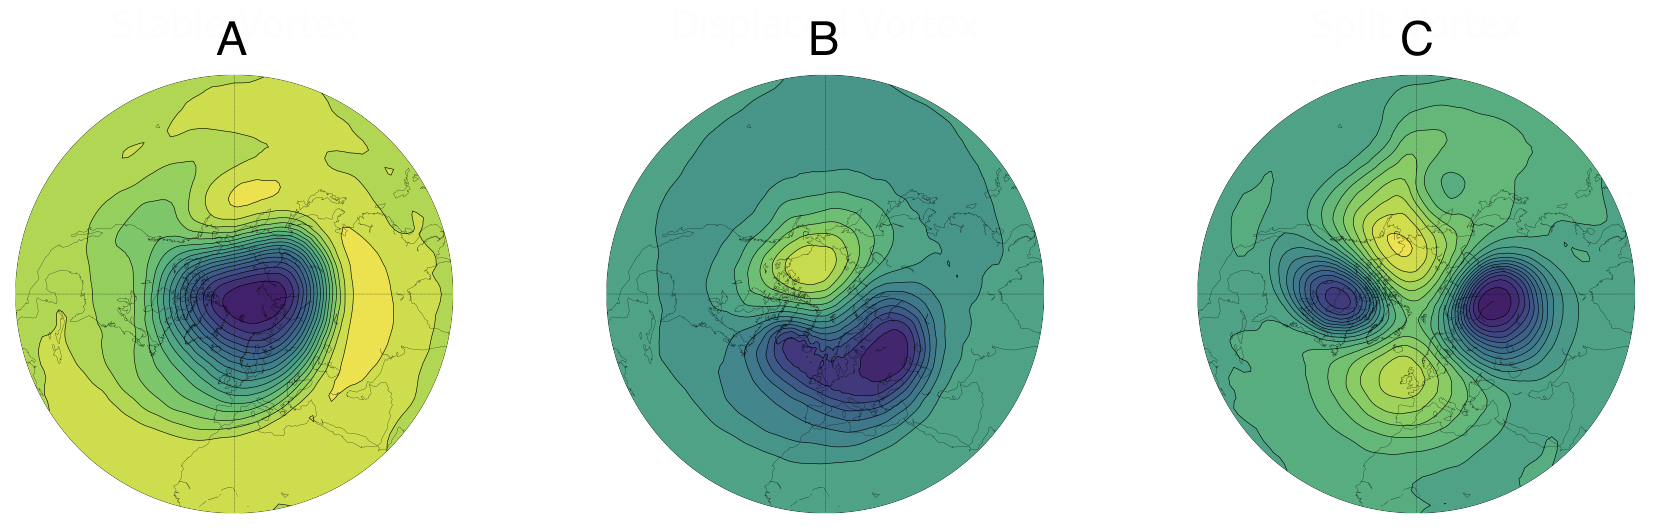
\includegraphics[width= \linewidth]{Figures/Figures-background/GPH_schematic.png}
\caption{10hPa geopotential Height over the NH hemisphere polar cap from ERA-interim showing three vortex configurations: Stable on 21/11/2008 (\textbf{A}), displaced on 22/02/2008 (\textbf{B}) and split on 24/01/2009 (\textbf{C}).}
\centering
\label{fig:GPH_schematic}
\end{figure}

It is shown in \cite{Seviour2013} that the type of deformation occurring broadly depends on the wavenumber of the dominant planetary waves involved with wave-1 disturbances more associated with displacement events and wave-2 with split events. Other studies utilising this vortex geometry approach note that SSWs are preceded by planetary wave breaking on the edge of the vortex in the so called "surf zone" which strips high PV air off the edge of the vortex thus sharpening its PV edge \citep{mcintyreBreaking1983}. Further works examine this phenomenon in the context of vortex preconditioning in which its geometry preceding SSWs promotes subsequent disruption. This geometry varies depending on whether the trigger for an event is considered as tropospheric wave bursts, in which case preconditions are generally a weak but westerly vortex which promotes propagation \citep{nishiiModulations2009b, kuttippurathComparative2012b}, or resonance with the stratospheric state in which case specific preconditions for split and displacement events are observed \citep{charltonNew2007c, bancalaPreconditioning2012b}. The framework provided by \cite{matsunoDynamical1971b} as well as insights from geometry analysis gives a picture of the processes involved in these remarkable dynamical events. The role SSWs play in two way stratosphere-troposphere coupling as well as their links to surface variability is discussed fully in sections \ref{sec:external_influence} and \ref{sec:Downward_influence}.

While many works into SSWs utilise observation based data, the observational record is relatively short (ERA-Interim is available from 1979-present) and general circulation models (GCMs) remain one of the most useful tools for developing understanding of the nature of these events. As a result, representing SSWs realistically in models is also key to this understanding. Multi-model comparisons of representation of SSW events have shown that large scale GCMs, including CMIP5 models, reproduce the polar vortex well but display a large degree of variation in SSW frequency \citep{Butchart2011, Kim2017}. Over the whole season, models with a well resolved stratosphere (high top) record higher numbers of SSWs and, unsurprisingly, a mean occurrence per season closer to reanalysis than those with a crude representation of the stratosphere (low top). However, there appears a significant overestimation of early winter warmings (November) in high top models compared to reanalysis \citep{Kim2017}. More recent studies utilising CMIP6 models report further variation in model SSWs and, in particular, disagreement across models in the response of SSW occurrence to anthropogenic forcing \citep{ayarzaguenaUncertainty2020b} which may originate from different treatment of physical processes underlying these events. \cite{Charlton2007} and \cite{Schmidt2013} show that most GCM’s struggle to obtain the correct sub-seasonal distribution of SSWs, with events occurring more uniformly across winter months compared to reanalysis in which the majority of events are recorded in January and February. The cause of this systematic bias is not well understood. A persistent past problem in the past with simulating seasonal SSW distributions was the so called "cold pole problem", with SSWs occurring too late in the season due to an overly strong early winter vortex \citep{pawsonGCM2000, Charlton2007}. This has largely been corrected by the introduction of improved gravity-wave parametrisation schemes \cite{garciaModification2017}. However, the schemes utilised in most GCMs are still relatively simple and there is a conflict between achieving a good representation of the polar regions (i.e. SSW frequency) and dynamical variability in the equatorial region (which are outlined in the following section). Both are forced through the gravity wave scheme. 

\section{The Equatorial Stratosphere}\label{sec:equatorial_strat}
Another region which exhibits key modes of stratospheric dynamical variability is the equatorial region. The most notable of these modes are the quasi-biennial oscillation (QBO) in the zonal flow which varies with a frequency of approximately 28-29 months between the 100\,hPa and 10\,hPa levels and the semiannual oscillation (SAO) of zonal wind which cycles more regularly with a frequency of 6 months around the 1\,hPa level (figure \ref{fig:QBO_SAO_ERA}) \citep{Baldwin1991}.

\begin{figure}[h!]
\centering
    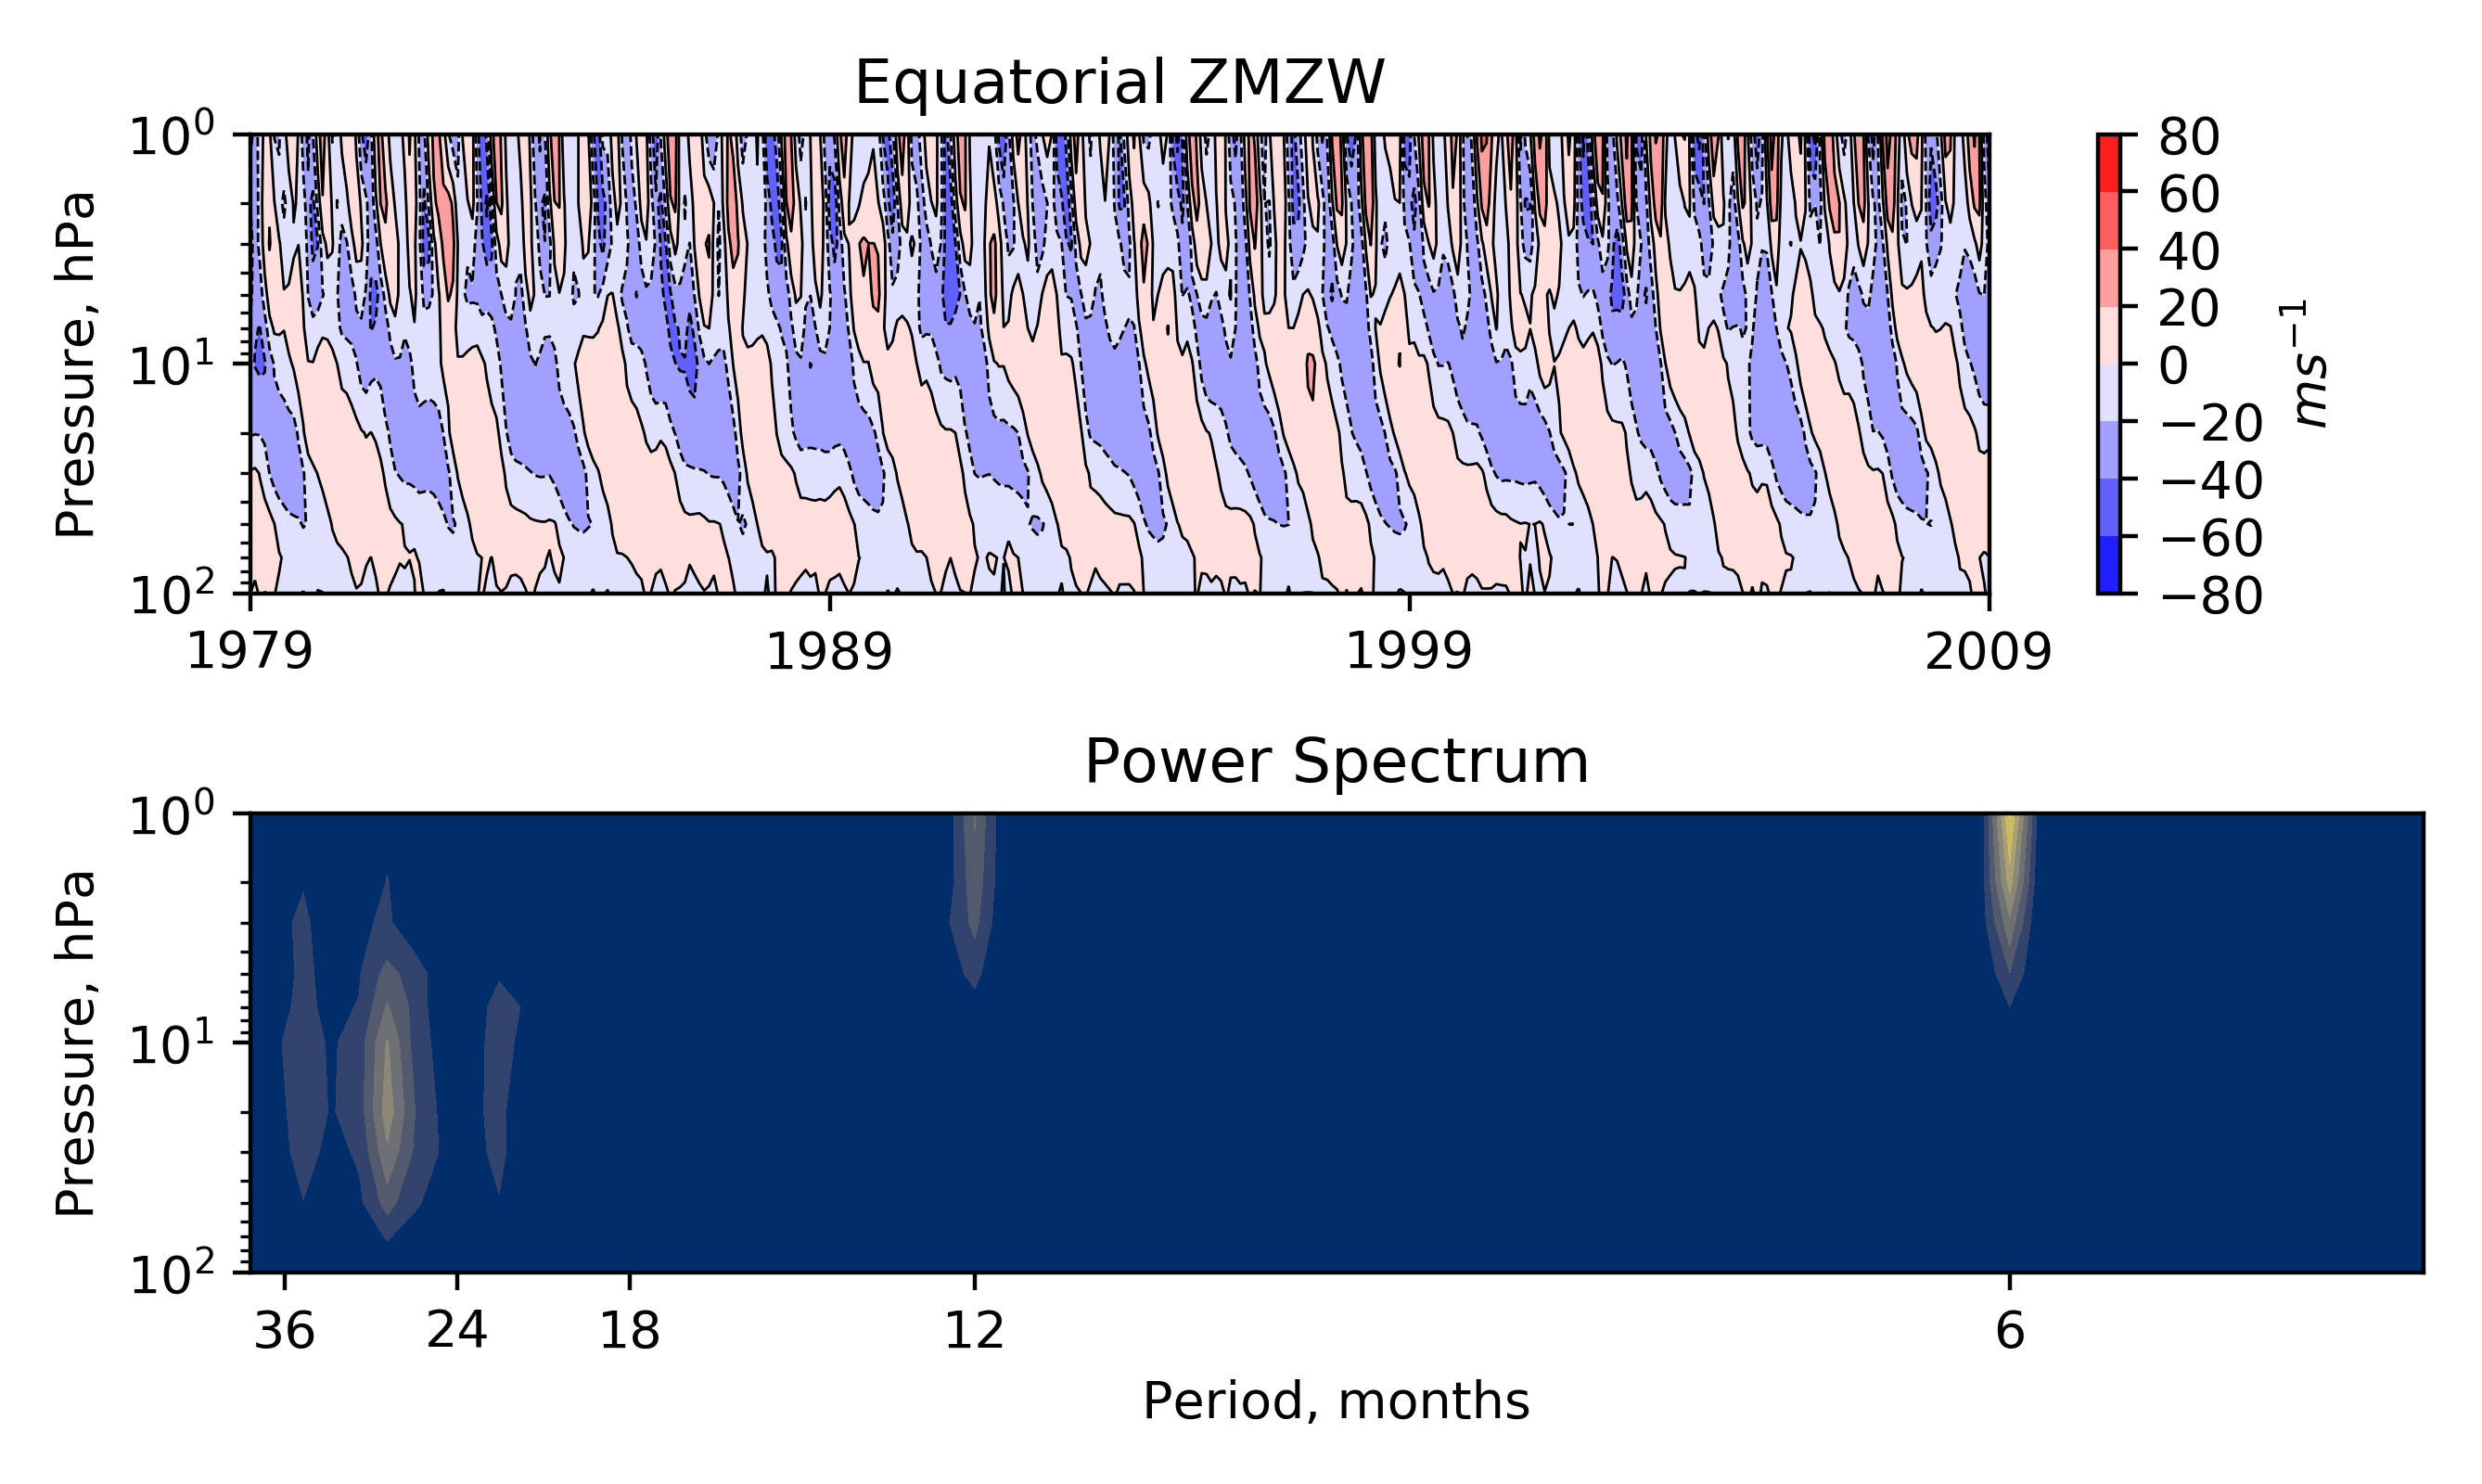
\includegraphics[width=0.88\textwidth]{Figures/Figures-background/QBO_SAO_ERA.png}
    \caption[Equatorial ZMZW and associated Fourier power spectrum from ERA-Interim.]{Equatorial ZMZW averaged between 5$^{\circ}$\,S--5$^{\circ}$\,N latitude(top) and associated Fourier power spectrum (bottom) from a 30 year sample from the ERA-Interim dataset between 1979 and 2009. A 30 year sample of data is provided to demonstrate the stalling of descending QBO phases.}
    \label{fig:QBO_SAO_ERA}
\centering
\end{figure}

The QBO was first fully classified as a phenomenon using balloon based observations in \cite{ebdonNotes1960, ebdonFluctuations1961} and \cite{reedQuasiBiennial1965}. These studies found a set of descending shears of easterly and westerly ZMZW above the equator between approximately the 10hPa and 100hPa pressure levels. These seminal studies made use of a short observational record (approximately 5 years) and later works with longer datasets were able to establish the key features of the oscillation \citep{baldwinQuasiBiennial2001,pascoeQuasibiennial2005b, schenzingerDefining2017}. These include an approximate period of 28.1 months (with a range of 22-40 months) and an asymmetry in the rate of descent of the westerly and easterly phases - slower descending easterly winds are caused by increased equatorial upwelling associated with this phase \citep{pascoeQuasibiennial2005b}. The oscillation is generally zonally symmetric \citep{belmontVARIATION1968} and has a latitudinal extent of approximately $12^{\circ}$ half width at half maximum \citep{baldwinQuasiBiennial2001}.

The primary cause of the oscillation is the interaction of waves outlined in section \ref{sec:atmos_waves} with the background zonal flow. To analyse the action of these disturbances, it is useful to consider a pair of equatorial waves with phase speeds of $+c$ and $-c$ respectively (figure \ref{fig:QBO_wave_schematic}, \cite{plumbQuasibiennial1984}). These waves propagate or dissipate according to the difference between their phase speed and the background flow, $\overbar{u}$. If $\overbar{u}$ approaches $+c$ or $-c$ at a given height, the respective wave will deposit momentum of the same sign as its phase speed onto the background flow. This means that, for a background wind profile like that shown in \ref{fig:QBO_wave_schematic}a, westerly momentum is deposited at the bottom of a zone of westerly low altitude background wind, while easterly phase speed waves pass through and are deposited above on easterly flow. This causes the shear zone to descend and reduces the width of the layer of the westerlies enough to allow viscous diffusion to eradicate the westerly winds completely near the surface. This leads to the profile in figure \ref{fig:QBO_wave_schematic}b where westerly waves pass through the flow and easterlies deposit momentum. Finally westerly waves begin to accelerate flow from high levels descending (as seen in schematic c) to finally force the background profile to figure \ref{fig:QBO_wave_schematic}d which is the inverse of schematic a. The asymmetry in descent speed between phases of the QBO is accounted for by the induced meridional circulation associated with each phase. An easterly QBO in the lower stratosphere induces a poleward meridional circulation at the same level \citep{plumbQuasibiennial1984, baldwinQuasiBiennial2001} as well as an acceleration in upwelling over the equator, this slows the descent of the QBO easterlies \citep{reedQuasiBiennial1965}. The converse is true for a westerly phase in the lower stratosphere.

Above the 10hPa pressure level, a different dominant mode of dynamical variability can be observed - the semi-annual oscillation (SAO) \citep{garciaClimatology1997}. This mode is categorised by two easterly and two westerly phases each calendar year with maximum amplitudes of approximately 30 $ms^{-1}$. These peak amplitudes are observed near the 1hPa level and also exhibit vertically descending shear zones like the QBO. While the QBO is purely driven by local equatorial wave-mean flow interactions, the SAO phases are driven by a combination of physical processes. The westerly phases, observed near the equinoxes, are thought to be caused by the action of a combination of Kelvin waves ($\sim$70\% of variability) and smaller scale inertia-gravity waves (the remaining $\sim$30\% of variability) \citep{dunkertonRole1979,hitchmanEstimation1988}. The easterly phase, observed at the two solstices, is the result of meridional advection of (summer hemisphere) easterlies from the Brewer-Dobson circulation \citep{holtonNumerical1980}. The easterly phases of the SAO also exhibit an asymmetry in amplitudes with the NH winter solstice phase stronger than its summer counterpart \citep{dunkertonRole1979}. This is due to a stronger Brewer-Dobson circulation in NH winter which leads to greater advection of easterlies to the equatorial region, leading to a stronger easterly SAO phase compared to NH summer. The periodicity of the SAO is therefore tied (through its easterly phase) to the seasonal cycle, unlike the QBO which has 'quasi-periodicity' because its period is determined by the amplitude of wave forcing. The westerly SAO phases show a similar asymmetry, NH winter westerlies are marginally weaker than their summer counterparts. This is due to increased gravity wave activity in NH autumn (Sep-Nov) compared to NH spring (Mar-Jun) \citep{rayAnalysis1998}. 

\begin{figure}[h!]
\centering
    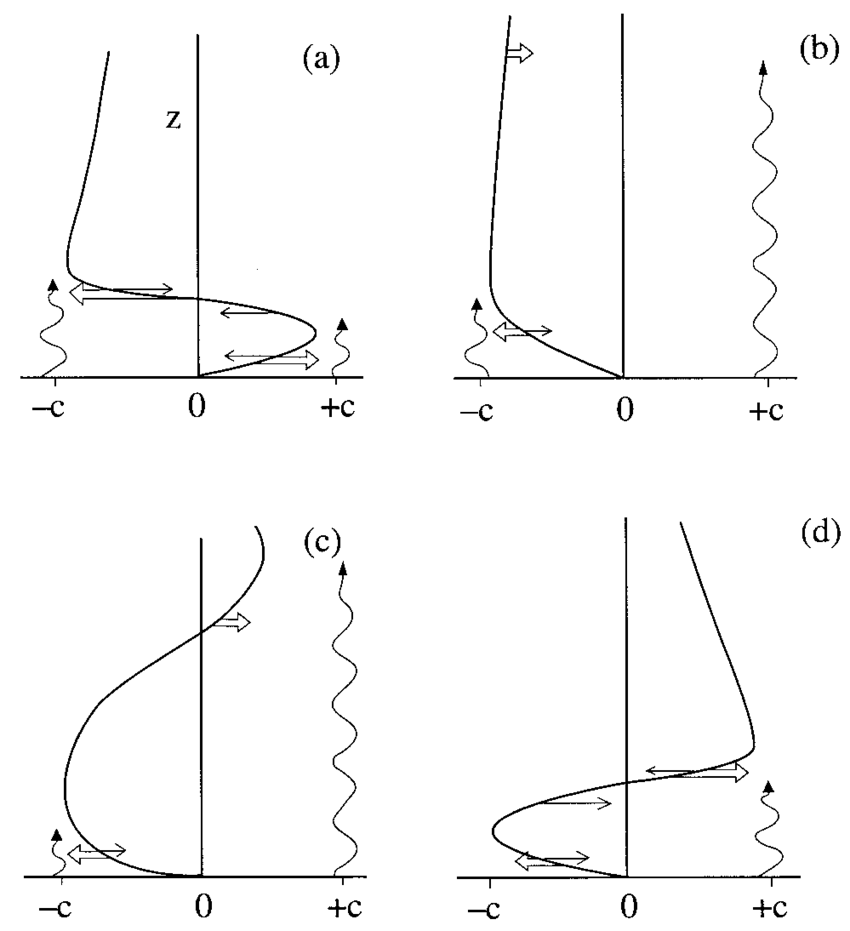
\includegraphics[width=0.5\textwidth]{Figures/Figures-background/Schematic_of_QBO_waves.png}
    \caption[Schematic of equatorial wave-mean flow interactions.]{Schematic of equatorial wave-mean flow interactions for two example wave disturbances (phase speeds $^+_- c$) from \cite{plumbQuasibiennial1984}. Solid continuous lines show the background flow of the QBO in developing phases, wavy arrows indicate propagation of the two waves, double arrows show momentum deposition on the mean flow from wave breaking, single arrows indicate viscous-driven acceleration.}
    \label{fig:QBO_wave_schematic}
\centering
\end{figure}

Significant research efforts have been conducted to understand and improve the representation of these equatorial modes of variability in GCMs. The first work to produce QBO like variability in a GCM was \cite{takahashiSimulation1996} yet subsequent works have highlighted the difficulty in reproducing this mode due to the specific set of conditions required for it to be simulated \citep{Baldwin2001}. Many studies have explored the importance of parameterised gravity waves for the production of a QBO and found them generally important \citep{giorgettaClimatology2006,ospreyClimatology2010b}. However, explicitly resolved waves were sufficient to produce a QBO in some high resolution simulations of the Model for Interdisciplinary Research on Climate (MIROC) \citep{kawataniQuasiBiennial2011}. Despite much research on the topic, only a small fraction of CMIP5 models captured an internally generated QBO-like variation \citep{charlton-perezLack2013}. As a result, the QBO initiative (QBOi) has been devised to produce a "recipe book for simulating a reliable QBO" using CMIP6 simulations and a set of standardised evaluation metrics \citep{butchartOverview2018}. Recent Work under the remit of the QBOi \citep{bushellEvaluation2020b} has suggested that the majority of CMIP6 GCMs exhibit a mean QBO period of near or less than the 28 months observed in reanalysis. The asymmetry in descent rates of easterly and westerly phases is not replicated successfully in some models, implying that the induced meridional circulation associated with the QBO may be problematic or that there may exist biases in the annual cycle in equatorial upwelling and its synchronisation with the QBO. Overall, the work suggests that the treatment of non-orographic gravity waves is the primary source of discrepancy in QBO across models \citep{bushellEvaluation2020b}. QBOi also considers representation of the SAO in its models. \cite{smithEquatoriala} presents representations from 11 models submitted to CMIP6 which vertically extend to the stratopause (the SAO region). These models are generally able to reproduce the seasonal variation (amplitude and phase) of winds compared to observations. However, the work notes that climatological winds of most models exhibit an easterly bias in the upper stratosphere which is attributed to an under-representation of small scale parameterised westerly phase speed waves. Despite the work of QBOi and other studies, there still remains significant open questions regarding representations of QBO and SAO in GCMs and how they might influence the vortex and SSW occurrence. How these equatorial modes interact with the vortex also remains a somewhat open question and is discussed in the following section. 

\section{External Influence on the Vortex}
\label{sec:external_influence}

While the NH vortex is confined to the NH stratosphere, variability in its strength can be influenced remotely by the troposphere, the surface and other parts of the stratosphere. The role of such influence on the vortex has been explored extensively in previous literature however the nature of dynamical coupling is not fully understood. 

\subsection{The Holton-Tan Effect}
\label{sec:external_influence_HT}

There exists a large body of literature examining the nature of the QBO and its interaction with the climate system; of particular relevance for the work presented in this thesis is how this mode couples with variability in the polar vortex. An association between the phase of the QBO and the strength of the polar vortex was first proposed by \cite{HoltonJamesRTan1980} and \cite{Holton1982} who found that the polar vortex exhibited a strengthening when the QBO near the 50\,hPa level was in its westerly phase (QBO-W) compared to its easterly phase (QBO-E). This link, usually referred to as the Holton-Tan (HT) effect, has been reported in subsequent studies with more comprehensive observations as well as in modelling studies using GCMs including the Met Office Hadley Centre Model 2 (HadGEM2) \citep{Watson2014} and other Met Office models \citep{Garfinkel2018}. Separate modelling studies also report a HT effect \citep{Baldwin1991,pascoeQuasibiennial2005b,luDecadalscale2008}.

A number of physical mechanisms have been proposed to account for the observed coupling between the QBO and the vortex. Most notable is the hypothesis that during westerly phases, the zero wind line (the latitude at various heights at which the NH mid latitude winter westerlies meet the summer easterlies) is shifted southwards \citep{HoltonJamesRTan1980}. This leads to a greater latitudinal dispersion of planetary wave activity as waves generated in the mid-latitudes are permitted to propagate vertically and equatorwards (according to the Charney-Drazin criterion, equation \ref{eq:Charney-Drazin}) thus decreasing their dissipative affect on the vortex. The converse argument can be made for easterly QBO phases when the zero-wind line lies further north and the planetary waves are guided more directly towards the vortex \cite{luMechanisms2014c}. Indications of this effect may manifest in EP-flux divergence at different latitudes for each QBO phase however, studies which have tested this mechanism show varied results. \cite{hamiltonEffects1998} finds a significant difference in latitudinal distribution of EP-flux divergence between QBO phases in accordance with the mechanism proposed above however \cite{huTropospheric2002} and \cite{graySolar2004} suggest the mechanism only takes effect during certain winter months, namely a stronger link is observed in early winter (Sep-Nov) compared to mid or late winter. Furthermore \citep{garfinkelDoes2012} present the idea of the HT effect competing with other phenomena such as the meridional circulation associated with QBO phases leading to variations in strength of QBO-vortex coupling. \cite{luMechanisms2014c} examines this further and shows that the strength of the HT effect is transient in nature; the coupling is weakened if a broader and stronger vortex is present in NH winter due to divergence of wave activity generated by eddies within the vortex itself. This diverts wave activity equatorwards, an opposite driving mechanism to that of Holton-Tan. These competing processes are thought to temporarily reduce the influence of the QBO on the vortex.

\subsection{The Aleutian Low}
\label{sec:external_influence_AL}

Vortex variability has also been closely associated with variations in winter surface climate that can determine the strength of mid-latitude tropospheric wave driving. Among the most notable of these is the climatological low pressure system over the Aleutian Islands in the Bering sea - the Aleutian low (AL). The AL is a key indicator of Pacific climate variability with teleconnections to both tropical and mid-latitude climate \citep{Nitta1989, Trenberth1994, zhangENSOlike1997} and it varies significantly on decadal to multi-decadal timescales \citep{overlandDecadal1999b}. The intensity of the AL has been shown to modulate vertical planetary wave propagation into the vortex region \citep{wooConnection2015b, garfinkelTropospheric2010b, manziniInfluence2006b}. Anomalously low pressure leads to an increase in Rossby wave amplitude with height \citep{wooConnection2015b} which can lead to stratospheric wave breaking and momentum deposition on the vortex associated with SSW occurrence. The effect has been found in the reanalysis study of \cite{huDecadal2018b} which attribute positive trends in vortex strength to a less intense AL and resulting weakening in wave-1 planetary wave flux into the stratosphere. Subsequent modelling studies report similar connections between AL indices and winter mean vortex strength as well as the the occurrence of SSW events \citep{krenWintertime2016b}. 

\subsection{ENSO and Tropical SSTs}
\label{sec:external_influence_SSTs}
Further surface features linked to vortex variability involve tropical sea surface temperatures (SSTs). For example the SST anomalies over the Eastern Pacific region associated with the El Ni\~{n}o Southern Oscillation (ENSO) have been shown to induce a stratospheric vortex circulation response via a pathway involving the AL \citep{domeisenTeleconnection2019d}. A positive ENSO phase is associated with a deepening of the AL (anomalously low pressures over the AL region) which promotes stronger planetary wave forcing of the middle atmosphere. This teleconnection has been found extensively in observation based studies \citep{garfinkelDifferent2008b, inesonRole2009b, smithLinear2012b} as well as modelling studies \citep{bellStratospheric2009b, domeisenSeasonal2015b, manziniInfluence2006b, richterEffects2015b}. However, the connection's robustness has also been shown to vary between ENSO events \citep{deserNorthern2017b, izaStratospheric2016b}, between decades \citep{ayarzaguena2018} and even within a single season (early vs late winter) \citep{ayarzaguenaIntraseasonal2018d} suggesting elements of non-stationarity in the teleconnection. Furthermore, there is a degree of asymmetry in the vortex response to anomalous positive (el Ni\~{n}o) and negative (la Ni\~{n}a) phases; SSWs occur at equal rates during winters of each ENSO phase and both at a higer rate than in neutral ENSO winters in the NCEP-NCAR reanalysis \citep{butlerNino2011b, garfinkelWhy2012b}. The elevated SSW rates during both ENSO phases are suggested to be due to sampling variability given the short observational record and further studies report a more linear ENSO-SSW connection in model simulations \citep{polvaniDistinguishing2017b} with no significant increase in SSW rates associated with La Ni\~{n}a winters in high-top CMIP5 models \citep{songRevisiting2018b}. El Ni\~{n}o winters' association with increased SSWs and a weaker winter vortex are consistent across model and observations \citep{manziniInfluence2006b, richterEffects2015b}. 

Additional studies consider the role of ENSO indices evaluated over different regions of the equatorial Pacific in coupling with the vortex. Two of these so called  "flavours" of ENSO variation are the central Pacific (CP) ENSO and the east Pacific (EastP) ENSO which are identified as separate modes of SST variability in the clustering analysis of \cite{johnsonHow2013f}. \cite{kaoContrasting2009d} also analyse these modes and show they represent the 1st (CP) and 2nd (EP) Empirical Orthogonal Functions (EOFs, see section \ref{sec:eof_analysis}), which indicate patterns of maximum variance, of interannual equatorial Pacific SST variations in the HadISST dataset. The same work finds that the EP pattern exhibits greater inter-decadal variability than its CP counterpart. Other works examine the teleconnections with the stratosphere associated with each type of pattern; \cite{izaRole2015b} examine vortex responses to patterns in a combined ERA-interim and ERA40 dataset and show significant correlation with both EP and CP ENSO indices. However the surface signal associated with CP el Ni\~{n}o conditions is more associated with a lower AL than the EP pattern in seasons where SSWs occur. Differences in vortex and mid-latitude wave activity responses to EP and CP patterns are also shown in modelling studies \citep{hegyiDynamical2011b} and in NCEP NCAR reanalysis \citep{sungAltered2014b}, highlighting probable differences in the physical mechanisms associated with each type of index. 

SSTs in other regions also exhibit elements of coherence with the vortex. \cite{raoVarying2018d} show that Tropical Atlantic SSTs give rise to a vortex response although it is highly variable throughout the season while \cite{fletcherRole2011b}, \cite{fletcherLinear2013b} and \cite{raoDecomposition2016b} propose a tropical Indian Ocean (TIO) connection: Positive TIO SST anomalies lead to a reduced strength of the AL that weakens the Rossby wave forcing of the vortex, an opposite effect to the ENSO-vortex connection where positive SST anomalies leads to vortex weakening. SST variability in the Northern Pacific basin, commonly labelled the Pacific Decadal Oscillation (PDO), has also been associated with the vortex (see section \ref{sec:PDO} for full details of this mode). The PDO has been shown to exert influence over stratospheric variability primarily through alteration of the AL with negative PDO phases associated with enhanced vertical and meridional propagation of planetary waves towards the vortex \citep{mantuaPacific1997a, rodionovSpatial2005b,raoModulation2019d}. This Association is reported in both observation and modelling based studies \citep{garcia-herreraPropagation2006b, krenWintertime2016b, huDecadal2018b}.


\section{Downward Influence of the Vortex}
\label{sec:Downward_influence}
So far, we have presented evidence for the influence of surface and tropospheric forcing on the vortex. Indeed, this was the sole view of stratosphere-troposphere coupling before the early 1990s when a selection of studies began to identify statistical coherence between vortex anomalies and subsequent patterns in the eddy-driven jet and NH surface patterns \citep{koderaDownward1990a,nigamStructure1990}. Since then, significant evidence has emerged in support of a two-way dynamical relationship between the atmospheric layers with influence of the stratosphere on modes of tropospheric and surface variability.

\subsection{The Northern Annular Mode}
\label{sec:NAM}

A key concept in the study of vortex and stratospheric influence on the troposphere and surface is that of the Northern Annular Mode (NAM). The NAM is regarded as the leading mode of dynamical variability in the NH extra-tropical atmosphere \citep{thompsonArctic1998, thompsonAnnular2000, baldwinPropagation1999} and is usually defined as the leading Empirical Orthogonal Function pattern (see section \ref{sec:stat_methods} for full details on EOF analysis) of NH geopotential heights (GPH) at various pressure levels \citep{baldwinPropagation1999}. The projection of this pattern onto the GPH fields gives a principle component (PC) index for the NAM. While these GPH fields are generally defined on 2D grids (in the latitude-longitude plane) many studies have been able to decrease computational expense by computing the NAM using zonal mean GPH fields \citep{baldwinCritical2009}. 

In the stratosphere, variations in the NAM broadly correspond to changes in winter vortex strength with the leading pattern resembling that of a strong, stable and zonally symmetric vortex \citep{baldwinPropagation1999}. On tropospheric pressure levels, variability in the strength and latitude of the tropospheric jet dominate \citep{limpasuvanEddies1999}. This makes the NAM a useful quantity for measuring the interactions between stratospheric and tropospheric variability as, in a single metric, it captures changes in distinct dynamical features of the NH winter stratosphere and troposphere (the vortex and the jet). The surface NAM pattern, often referred to as the Arctic Oscillation (AO), resembles the well known dipole structure over the Atlantic, the North Atlantic Oscillation (NAO) \citep{hurrellNorth2003c}. This mode consists of two centres of action over the Azores and Icelandic regions which are displayed in figure \ref{fig:AO}a. In addition to the NAO characteristics, the surface NAM also exhibits a centre over the AL region in the North Pacific. There is some debate regarding the relative roles of the NAO and AL sections of the AO pattern. Namely, whether the two features are truly coupled or can exist independently \citep{deserTeleconnectivity2000, ambaumArctic2001} as well as how this may change under under anthropogenic forcing \citep{hamoudaDecoupling2021}. The AO pattern is shown in figure \ref{fig:AO}a along with the corresponding PC index.

\begin{figure}[h!]
\centering
    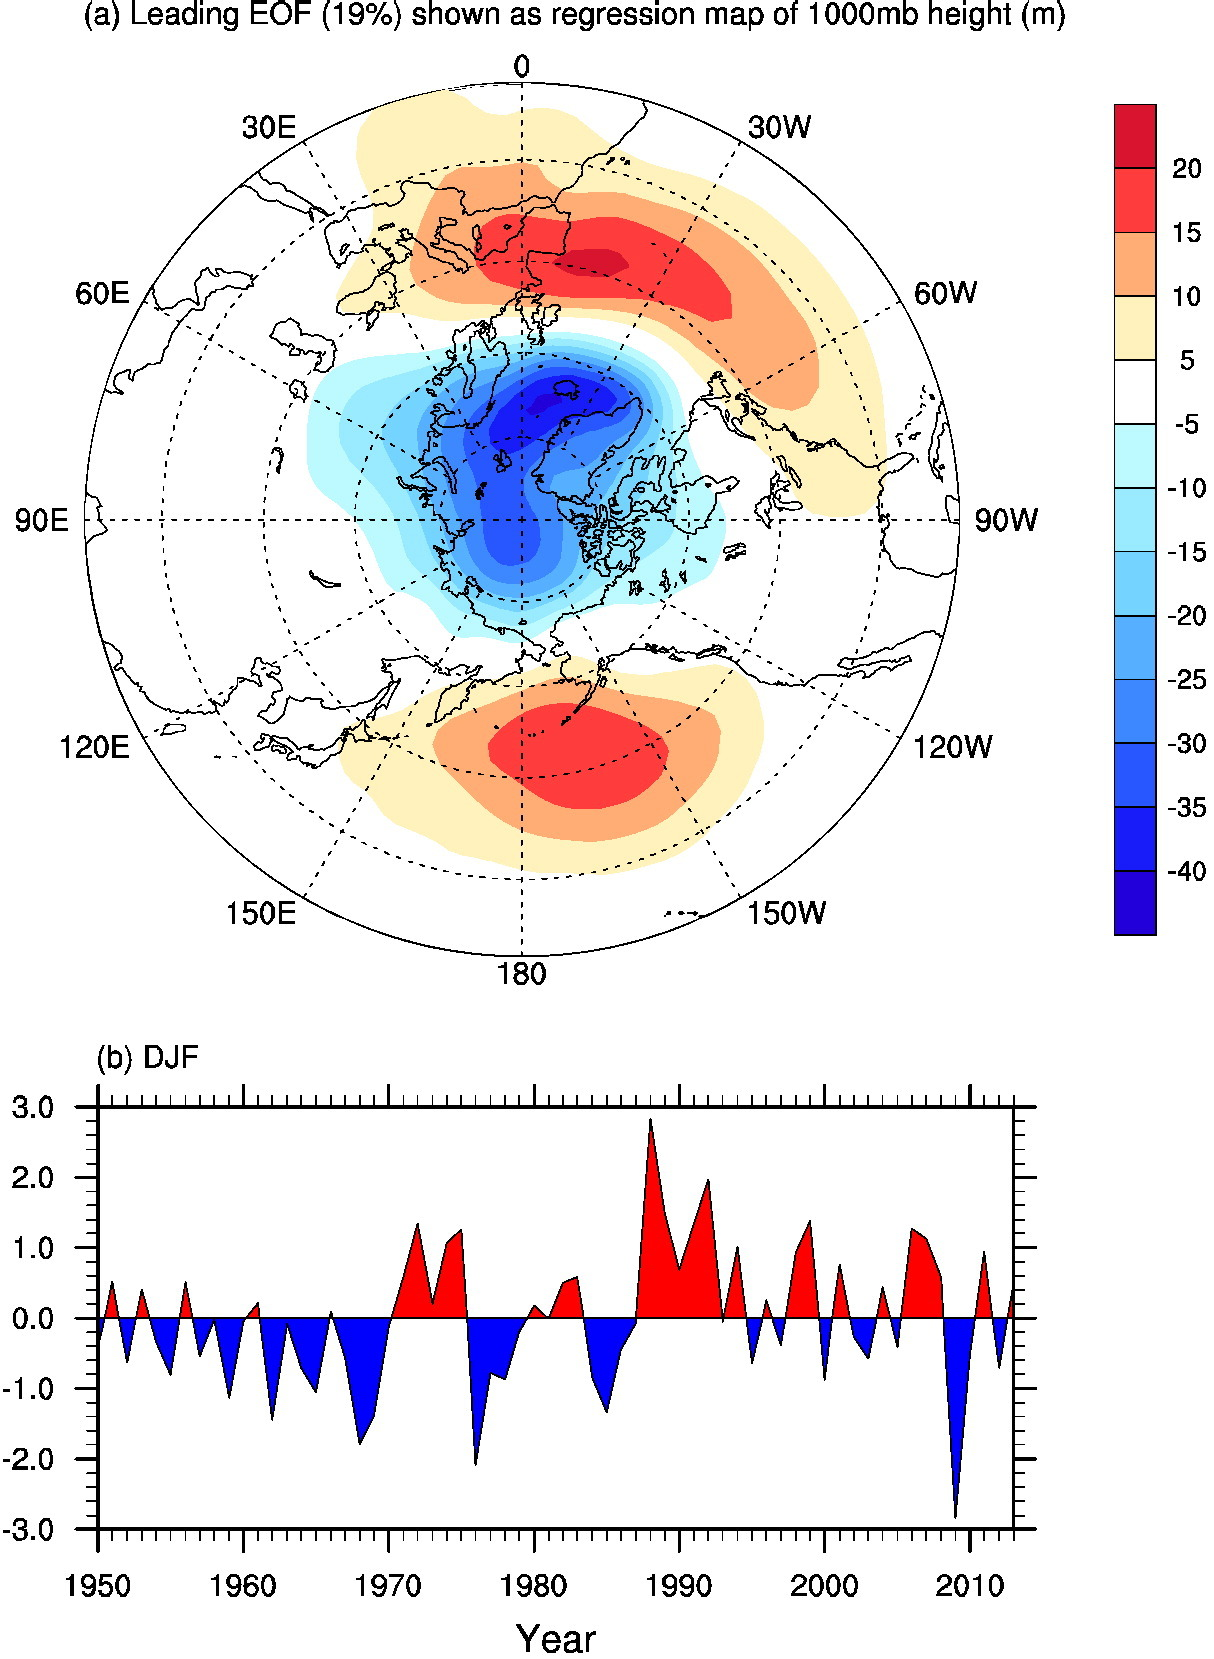
\includegraphics[width=0.5\textwidth]{Figures/Figures-background/AO_pattern.jpg}
    \caption{The Surface NAM pattern (also referred to as the Arctic Oscillation) derived by \cite{hegyiDynamical2011b} using GPH data from the NCEP/NCAR (National Center for Environmental Prediction/National Center for Atmospheric Research) reanalysis dataset. \textbf{(a)} shows the leading EOF pattern of monthly mean GPH on the 1000hPa level from the 1979-2000 period. The percentage quoted in parenthases indicates the fraction of the variance in GPH explained by the lead EOF. \textbf{(b)} shows the principal component timeseries generated by projecting the pattern in \textbf{(a)} onto the winter (Dec-Feb) GPH anomalies from the same dataset.}
\centering
\label{fig:AO}
\end{figure}


\subsection{Tropospheric and Surface Variability}
The notion of vortex influence over tropospheric and surface climate variability was first fully analysed in the seminal work of \cite{baldwinStratospheric2001a} which demonstrated a steady downward propagation of NAM anomalies from the middle stratosphere to the surface following strong and weak vortex events (SSWs) in the ERA40 reanalysis dataset (figure \ref{fig:Baldwin_composite}). The surface perturbations associated with an anomalous vortex were shown to persist intermittently for approximately 60 days after the event and project significantly onto the negative pattern of the NAO and AO. Subsequent studies have corroborated these results: \cite{domeisenEstimating2019d} show using ERA40 and ERA-Interim datasets that approximately 2/3 SSW events are followed either by a switch from positive to negative NAO or a persistent negative NAO pattern. \cite{charlton-perezInfluence2018e} consider this coupling from the perspective of tropospheric weather regimes and find, in both ERA-Interim and the ECMWF Integrated forecast model, a 40-60\% increase in probability of transition to a negative phase of the NAO given a 1 standard deviation reduction in polar vortex strength. SSWs' projection onto negative NAO phase probability has subsequently been shown to influence NH winter temperatures.

\cite{thompsonStratospheric2002b} show in NCEP–NCAR reanalysis that SSWs are followed by a 60 day interval of anomalously low surface temperatures in eastern North America, northern Europe, and eastern Asia. Subsequent observational studies find similar response patterns to SSWs \citep{kolstadAssociation2010b, kingObserved2019b, lehtonenObserved2016b} and the effect can also be seen in GCM simulations \citep{tomassiniRole2012b, lehtonenObserved2016b}. Equally, the absence of an SSW, when the vortex is relatively undisturbed by waves propagating from the troposphere so that the vortex is unusually strong and cold, also has significant impacts on surface weather \citep{shawLife2013b, lawrenceRemarkably2020b}. Further impacts of SSWs on tropospheric circulation include an equatorward shift and deceleration of the North Atlantic eddy-driven jet stream which correspond to negative tropospheric NAM anomalies \citep{hitchcockDownward2014b,maycockRegime2020b}. Links with persistent blocking events are also shown in observation and modelling studies \citep{daviniBlocking2014b, vialSudden2013b} although \cite{taguchiThere2008b} finds no significant link between the phenomena.

\begin{figure}[h!]
\centering
    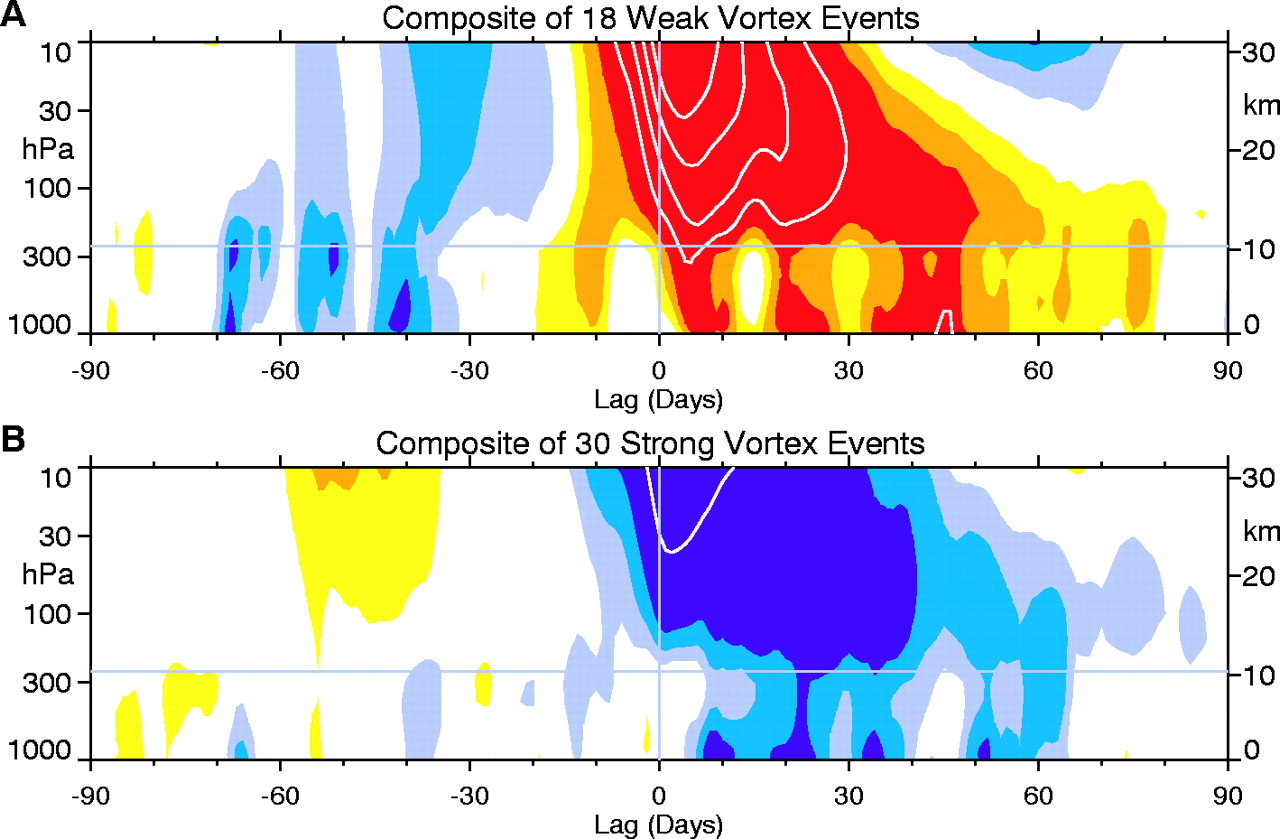
\includegraphics[width=0.7\textwidth]{Figures/Figures-background/baldwin_composite.jpg}
    \caption[Time-height composites of the NAM about anomalous vortex events in the ERA40 dataset from \cite{baldwinStratospheric2001a}.]{Figure from \cite{baldwinStratospheric2001a}: Time-height composites of the NAM about anomalous weak (A) and strong (B) vortex events in the ERA40 dataset. Events are defined when NAM values cross -3.0 (weak) and +1.5 (strong). Coloured contours are spaced at 0.25 NAM intervals while white contours are spaced at 0.5. Only NAM values with a magnitude greater than 0.25 are shown. Vertical lines denote the central date of the vortex event and horizontal lines the approximate height of the tropopause.}  
    \label{fig:Baldwin_composite}
\centering
\end{figure}

Although the composite analysis of \cite{baldwinStratospheric2001a} indicates an average downward propagation of stratospheric anomalies, the same work demonstrates that only a fraction of vortex events perturb tropospheric and surface NAM signals. The cause of this fraction is not fully understood: \cite{Mitchell2011} and \cite{Seviour2016} propose, using reanalysis and CMIP5 model data, that split vortex events have a greater probability of penetrating through the tropopause and exhibit a larger response at the surface than displacement events. However, \cite{Maycock2015} carry out a similar analysis on a large ensemble of pre industrial control model runs (1000 years worth of simulation) and find no statistically significant difference between the vertical profiles of the two event types. Other works suggest that increased wave activity in the mid to lower troposphere preceding an event can influence its downward impact. \cite{Nakagawa2006} demonstrate anomalously high wavenumber two activity associated more with propagating events while \cite{White2019} find that 2/3 of events preceded by enhanced planetary wave activity in the lower troposphere are propagating. However, the authors acknowledge that this attribute could not be used deterministically to predict whether a given event will propagate into the troposphere. Despite the lack of full understanding regarding downward propagation of vortex events, their influence on surface patterns is relatively well represented in modern GCMs \cite{baldwinSudden2021b}. Idealised modelling studies using the Model of an Idealized Moist Atmosphere (MIMA)  are able to show a direct downward influence of SSW events on the NAO by imposing disturbed vortex conditions and measuring the surface response \citep{whiteGeneric2020b}. Similar results are obtained in \cite{gerberStratospheric2009b} which utilises a similar method. However, some works note that simple models tend to over-represent the persistence of surface anomalies \citep{gerberAnnular2008b, gerberTesting2008b} indicating that a complex combination of factors not captured by simplified model setups likely cause the varying degrees of propagation for different SSWs. 

\section{Multi-decadal Climate Variability}
\label{sec:multi-decadal_background}
In the majority of studies covered thus far, the vortex and its interactions with the the wider climate system are considered within each NH winter, and variability in its strength is considered primarily on interannual timescales. However, there is a growing body of evidence in support of modes of variability on multi-decadal timescales in the climate system. Here, we outline some of the most well studied of these modes. 

\subsection{Atlantic Variability}
A domain often associated with multi-decadal timescale variations is the ocean, primarily due to the high degree of thermal inertia present in ocean systems. One of the primary modes of variability in ocean circulation is the Atlantic Meridional Overturning Circulation (AMOC) which consists of a northward transfer of warm, saline water that occurs in the top 2km of the Atlantic Ocean (the "upper cell") accompanied by a corresponding return flow of southward transport at lower depths, the "lower cell" often referred to as the North Atlantic Deep Waters (NADW) \citep{kuhlbrodtDriving2007b, xuIntraseasonal2014b, buckleyObservations2016d}. The AMOC is thought to be a key driver of North American and European surface variability via modulation of Atlantic sea surface temperatures (SSTs) and heat transport \citep{knightSignature2005b, delworthObserved2000b, friersonContribution2013b, frankignoulInfluence2013b}. It has been shown to influence a diverse range of features such as European summertime temperatures \citep{suttonAtlantic2005b}, biogeochemical conditions in the northwest Atlantic \citep{lavoieProjections2019b} as well as abrupt climate shifts in paleoclimate records \citep{alleyWally2007c, chengIce2009c}. 

The strength of the AMOC has been shown to vary significantly on decadal-centennial timescales \citep{delworthInterdecadal1993b, biastochCauses2008c, tullochExploring2012b, menaryMultimodel2012b}. \cite{biastochCauses2008c} show, using a suite of ocean models with varying resolutions, that these characteristic timescales are likely due to the complex interaction of different driving mechanisms including wind and thermohaline forcing as well as subarctic deep water formation which is transferred to the tropical Atlantic. Both modelling and observational studies link the AMOC to the Atlantic Multidecadal Variability (AMV), a prominent mode of variability in subpolar North Atlantic SSTs with a period of 60-80 years in observations \citep{zhangReview2019}. For example, the observation based study of \cite{mccarthyOcean2015} shows that the decadal scale changes in the AMOC lead to similar fluctuations in the AMO through alterations in subpolar gyre heat content, a finding that backs up the earlier modelling study of \cite{delworthObserved2000b} which proposed a similar mechanism.

Multiple potential drivers of AMOC variability at different timescales have been studied extensively in both observations and modelling studies. On intra-annual to inter-annual timescales, variability in the AMOC has been closely associated with wind variations over the North Atlantic region through Ekman-transport anomalies or wind stress curl forcing \citep{wangCharacteristic2019b, mccarthyObserved2012b, mielkeObserved2013b, yangLocal2015b}. On inter-annual to decadal timescales, AMOC variability has been associated with buoyancy anomalies in the subpolar region, particularly in the Labrador Sea \citep{delworthInterdecadal1993b, medhaugMechanisms2012b}. This mechanism is linked to variability in mixed layer depth and the occurrence of deep convection over the same region, particularly in NH winter \citep{boningDecadal2006c, biastochCauses2008c, robsonCauses2012c, wangVariability2015b}. Mixed-layer anomalies in the Labrador Sea are an indication of the strength of deep convection in this region, which has been shown to be associated with AMOC variations in modelling studies \citep{edenMechanism2001b, edenNorth2001b} and observations \citep{latifPerspective2011b}.

Recent studies focussed on the observed AMOC have shown a negative trend in circulation strength of approximately $-2.7 Sv$ ($1 Sv = 10^6 m^3 s^{-1}$) between 2004 and 2012 \citep{smeedNorth2018b} before a marginal recovery after 2012 \citep{smeedAtlantic2019c}. Modelling studies have proposed a key role for anthropogenic forcing in AMOC slowdown over the 20th century and into the future \citep{liuOverlooked2017a, bakkerFate2016b, liuMechanisms2019b} however the magnitude of this contribution as well as others carries significant uncertainties. Research efforts into understanding these AMOC trends rely heavily on GCMs and subsequently their representation of the AMOC. Recent studies (e.g. \cite{robsonEvaluation2020d}) evaluate the representation of the AMOC in a modern GCM (the UK Earth System Model in this case) and find it is able to realistically simulate key features of the AMOC over the historical period but under-represents decadal scale variability compares to observations. It also underestimates the size of the recent trends reported in \cite{smeedNorth2018b, smeedAtlantic2019c}. The same issue is reported in a suite of CMIP5 models in \cite{roberts20042014}.

\subsection{Pacific Variability}
\label{sec:PDO}
An analogous mode of SST variability to the AMV can be observed in the Pacific basin labelled the Pacific Decadal Oscillation (PDO, \cite{mantuaPacific1997a}). This mode is often defined using the leading EOF and associated PC of north Pacific SSTs (however a simpler box average over the same region index is also utilised). This mode is shown to exhibit spectral power at a range of frequencies in a suite of CMIP5 models which show little consensus as to the characteristic timescale of variations \cite{newmanPacific2016}. Other studies into the spectral features of the PDO report significant non-stationary regime behaviour \citep{overlandRegime2006, flemingNonuniqueness2014} as well as variations between 20 and 70 year periods utilising paleoclimate proxy records \citep{biondiNorth2001}. Despite these works, there remains an open question as to the true characteristic timescale of PDO variations and \cite{newmanPacific2016} suggest this is likely because this mode is not simply a single phenomenon but the result of a complex combination of physical processes. 

A variety of mechanisms are proposed to drive PDO variations. For example, \cite{frankignoulStochastic1977} show a possible role of stochastic atmospheric forcing (effectively white noise) from the AL region whose effect is integrated over time due to the longer memory of the ocean. Links to the tropical Pacific are also explored with \cite{strongRole2009} showing an influence of ENSO SSTs via modulation of the AL particularly in boreal winter (when ENSO peaks). The ENSO-PDO connection may also contribute to decadal timescale fluctuations in the PDO as \cite{alexanderAtmospheric2002, alexanderRole2008} show using GCM integrations that 1/4-1/2 of PDO variability originate in the tropical Pacific. Low frequency (longer than a decade) co-variability between ENSO and the PDO is also shown in other observational and modelling studies \citep{vimontContribution2005, chenENSOLike2015}.

The PDO has been shown to influence stratospheric variability primarily through alterations in AL intesnsity and subsequent modulation of planetary wave driving of the vortex \citep{krenWintertime2016b,Kang2017,huDecadal2018b}. PDO and ENSO like SST variations have been shown to perturb the vortex in numerous modelling studies \citep{krenWintertime2016b,garcia-herreraPropagation2006b}) however the role of decadal scale variations in such teleconnections is less well explored and is one of the aims of the original work presented in this thesis.

The set of modes outlined in this section is not exhaustive within the climate system however the AMOC, AMV and PDO represent some of the most well studied features which exhibit variations on this timescale. The aim of analysis in chapters 3 and 4 is to determine whether the vortex and equatorial stratosphere exhibit similar multi-decadal variability as well as to establish how these signals may interact with the modes outlined above.



